\section{Descrizione del progetto}
Per quanto riguarda la parte di \textit{ASM} si è deciso di riprendere un esempio visto in classe (e durante le pause caffè, molto amate da noi studenti), ovvero quello relativo alla \textit{\textbf{Coffee machine}}, che affiancherà il distributore di bevande energetiche progettato in Scala.

In particolare l'applicazione è stata definita basandosi su una serie di specifiche, quali:
\begin{itemize}
	\item Il distributore modellato può preparare \textbf{diverse tipologie di bevande} (caffè, cappuccino etc), ognuna delle quali è preparata con diverse quantità di ingredienti (acqua, caffè, latte etc) i quali vengono consumati dagli utenti;
	\item Il distributore accetta \textbf{pagamenti solamente in moneta} tramite l'inserimento di denaro nell'apposita fessura;
	\item Il distributore è in grado di fornire il resto;
	\item Quando tutte gli ingredienti sono esauriti, il distributore va fuori servizio, in attesa che gli ingredienti vengano aggiunti dal manutentore (\textbf{questa parte non è però stata modellizzata nella presente ASM}).
\end{itemize}
	

\section{Macchina a stati}
La ASM è basata su una macchina a stati finiti, mostrata in figura ~\ref{fig:StateMachine}, che definisce i principali stati e le principali transizioni che si possono verificare durante il funzionamento del distributore. 
\begin{figure}[h!]
	\centering
	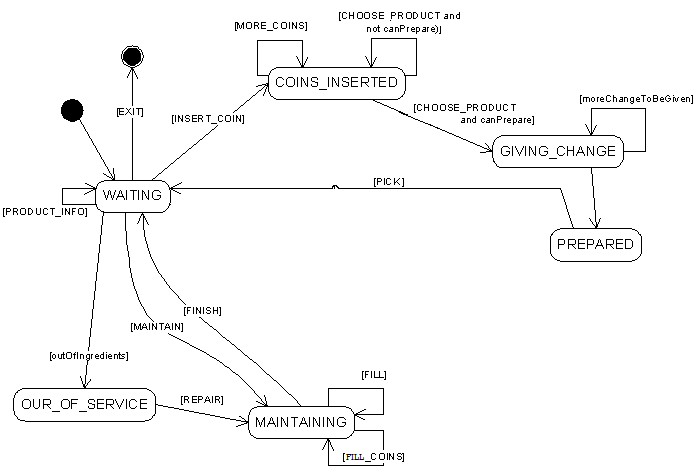
\includegraphics[width=0.6\textwidth]{Immagini/FSM.png}
	\caption{Macchina a stati}
	\label{fig:StateMachine}
\end{figure}

\newpage
\section{Eventi}
La ASM sviluppata modella un sistema event-driven, ovvero un sistema in cui le transizioni da uno stato all’altro sono perlopiù scatenate da input dell’utente, mentre di solito la macchina si trova ferma in uno stato, in attesa di tali eventi.

Nel codice ASMETA questi eventi sono denominati \textbf{action}: ad ogni stato corrispondono una o più azioni che l’utente può compiere quando la macchina si trova in quello stato, le quali sono codificate come elementi di un dominio enumerativo (figura ~\ref{fig:actionASM}).

\begin{figure}[h]
	\centering
	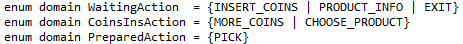
\includegraphics[width=0.6\textwidth]{Immagini/ActionASM.png}
	\caption{Action che implicano un possibile cambio di stato, qualora la condizione sia verificata}
	\label{fig:actionASM}
\end{figure}

La caratteristica event-driven del sistema si è riflessa nella ASM, infatti le regole (\textit{rules}) implementate possono essere suddivise in due categorie:
\begin{itemize}
	\item  regole che attendono il verificarsi di un’azione (qui chiamate \textbf{event management rules});
	\item regole di transizione (\textbf{transition rules}) che verificano la \textbf{condizione} (spesso chiamata anche \textbf{guardia}) della transizione e, se verificata, eseguono gli update opportuni per effettuare il passaggio di stato. Esse possono infatti essere viste come istruzioni del tipo 
	
	\textit{\textbf{if} Condition \textbf{then} Update}.
\end{itemize}
	
\textbf{In linea di massima, ad ogni stato corrisponde una \textit{event management rule}, mentre ad ogni arco (transizione) corrisponde una \textit{transition rule}.}

\section{Domini}
I domini introdotti nel codice ASM sono:
\begin{itemize}
	\item \textbf{Domini enumerativi}: per gli stati della FSM, uno per ciascun insieme di eventi (ciascun insieme contiene gli eventi validi per uno stato), ovvero quelli relativi alle possibili azioni eseguibili in ogni specifico stato, ed uno relativo alla tipologia di ingredienti utilizzati (figura ~\ref{fig:enumDomain});
	\item \textbf{Dominio statico concreto} per i tagli di monete riconosciuti dal distributore (in centesimi);
	\item \textbf{Dominio astratto} per i prodotti erogabili dal distributore.
\end{itemize}

\begin{figure}[h]
	\centering
	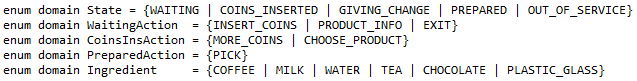
\includegraphics[width=0.5\textwidth]{Immagini/EnumDomain.png}
	\caption{Domini enumerativi}
	\label{fig:enumDomain}
\end{figure}

\newpage
\section{Static and Dynamic functions}
\subsection{Static}
Le funzioni static (figura ~\ref{fig:staticFunc}) sono funzioni la cui interpretazione viene fissata dalla definizione della ASM e non può essere modificata durante l’esecuzione: questo significa il valore che forniscono come risultato non dipende dagli stati attuali della ASM, e quindi dalla sua dinamica.

Possono essere paragonate alle costanti dei linguaggi di programmazione classici.
\begin{figure}[h]
	\centering
	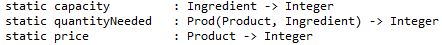
\includegraphics[width=0.5\textwidth]{Immagini/StaticFunction.png}
	\caption{\textit{Signature} delle static functions utilizzate}
	\label{fig:staticFunc}
\end{figure}

Per esempio la funzione \textit{price} rappresenta un legame costante tra un prodotto e il suo prezzo, e sarà sempre lo stesso, sia nel caso in cui ci si trova nello stato di "\textit{monete inserite}" che nel caso di stato pari a "\textit{out of service}"

\subsection{Dynamic}
La funzioni dinamiche, a differenza di quelle statiche, dipendono dallo stato in cui l'ASM si trova, e quindi andranno a fornire una risposta diversa a seconda di quelle che sono le condizioni in cui si trova la macchina a stati.
Le funzioni dinamiche sono a loro volta suddivise in 4 sotto-classi: nella applicazione realizzata sono state utilizzate le funzioni di tipo \textit{controlled} e \textit{monitored}.

\subsubsection{Controlled}
Le funzioni in figura ~\ref{fig:controlled}, rappresentano funzioni dinamiche di tipo \textbf{controlled} così definite:
\begin{figure}[h]
	\centering
	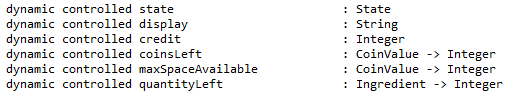
\includegraphics[width=0.65\textwidth]{Immagini/DynamicController.png}
	\caption{Funzioni dynamic - controlled}
	\label{fig:controlled}
\end{figure}

Si vede come le prime tre funzioni rappresentino delle \textbf{funzioni 0-arie}, ovvero delle variabili.

Le ultime tre invece sono \textbf{funzioni n-arie}, ovvero mappano dei valori (come in una tabella) da un dominio ad un codominio: nell'applicazione abbiamo creato 3 funzioni n-arie presentate di seguito:
\begin{itemize}
	\item \textbf{coinsLeft}: associa ad ogni taglio di moneta il numero attuale di monete presente all'interno del distirbutore;
	\item \textbf{quantityLeft}: ad ogni tipologia di ingrediente associa un valore Integer, che non è altro che la quantità rimasta.
\end{itemize}

I valori assunti dalle funzioni controlled rappresentano parte dello stato esteso delle ASM, quindi possono essere utilizzate per mantenere informazioni tra uno stato e l’altro della FSM.

\subsubsection{Monitored}
Le funzioni monitored rappresentano degli input che l’utente fornisce alla macchina: esse infatti sono funzioni che sono lette ma non sono state aggiornate dalla ASM.

Il valore di queste funzioni non è persistente, ma viene ad essere specificato dall’utente per ogni stato tramite tastiera (oppure letto anche da file esterno, come fatto per i test automatici tramite file).


\begin{figure}[h]
	\centering
	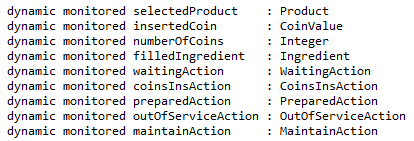
\includegraphics[width=0.65\textwidth]{Immagini/MonitoredFunc.png}
	\caption{Monitored functions}
	\label{fig:monitoredFunc}
\end{figure}

Tra le funzioni monitored figurano le funzioni che richiedono all’utente la scelta di quale azione deve compiere il distributore tra l'insieme di azioni disponibili.

Inoltre ci sono funzioni con cui l’utente specifica quale moneta, quale prodotto è stato selezionato.

\section{Event management rules e main rule}
Le event management rules si occupano di ricevere le azioni dell’utente e di eseguire la regola di transizione opportuna. 

In figura ~\ref{fig:managementRules} c’è un elenco delle regole, la cui struttura è del tutto simile a quella delle altre regole definite.

\begin{figure}[h]
	\centering
	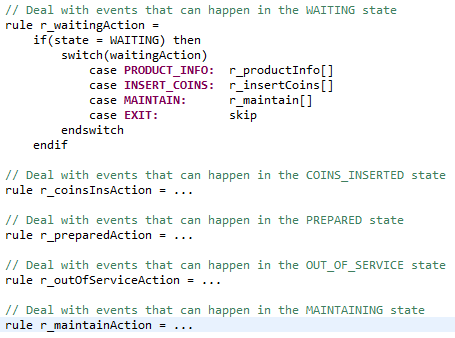
\includegraphics[width=0.5\textwidth]{Immagini/ManagementRule.png}
	\caption{Management rules}
	\label{fig:managementRules}
\end{figure}

La \textit{main rule}, che costituisce l’entry point del programma, controlla per prima cosa che il distributore possa operare, ovvero che non abbia finito gli ingredienti (r-selfCheck); questo è possibile grazie al comportamento del blocco sequenziale, che effettua gli update dopo la valutazione di ciascun termine.

Dopo il controllo, invece, vengono valutate in parallelo le regole di gestione degli eventi: per esse non vi è pericolo di \textit{update inconsistenti} perché ciascuna regola ha una guardia che permette di valutare la regola solo quando la macchina si trova nello stato corretto (ogni regola si applica a un diverso stato, quindi sola una alla volta è “attiva”).

\section{Inizializzazione}
Perché la macchina inizi a operare in uno stato diverso, più significativo (anche perché raramente la macchina viene definita in modo da poter gestire valori undef), deve essere inizializzata, ovvero definirè necessario definire uno stato iniziale, come fatto in figura ~\ref{fig:initialState}

\begin{figure}[h]
	\centering
	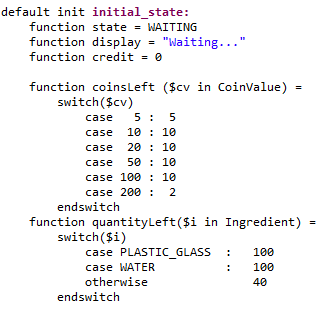
\includegraphics[width=0.5\textwidth]{Immagini/InitialState.png}
	\caption{Inizializzazione}
	\label{fig:initialState}
\end{figure}

In questo caso:
\begin{itemize}
	\item lo stato FSM iniziale è quello di attesa (\textit{function state = WAITING});
	\item il credito in monete è nullo (\textit{function credit = 0});
	\item  la macchina possiede un discreto quantitativo di monete e ingredienti (chiamata delle funzioni n-arie dinamiche), per poter operare per un certo periodo senza bisogno di manutenzione.
\end{itemize}

\section{Simulazione}
La macchina è stata simulata con AsmetaS, sia in modalità interattiva che in modalità batch.
In modalità interattiva è facile scoprire errori sia di transizione di stato FSM sia di update, perché ad ogni update viene mostrato lo stato completo. 
Un esempio di simulazione interattiva è riportata di seguito (figura ~\ref{fig:iterativeExe}): in questo esempio abbiamo provato a prendere un caffè da una distributore che aveva ingredienti sufficienti solamente per un caffè. Come si vede infatti, il distributore è andato, dopo aver erogato il prodotto, in stato \textit{OUT OF SERVICE}, terminando l'applicazione.

\begin{figure}[h]
	\centering
	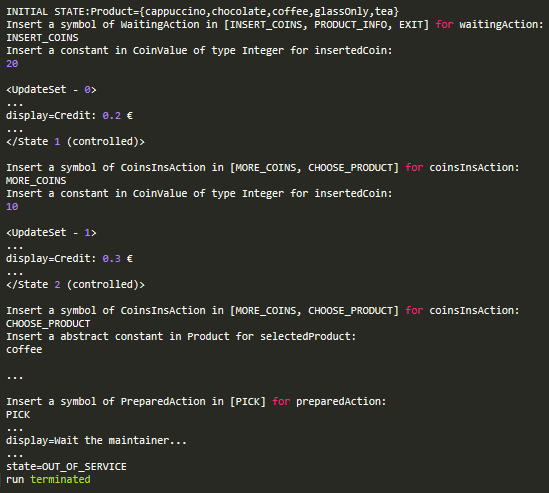
\includegraphics[width=0.5\textwidth]{Immagini/IterativeRunASM.png}
	\caption{Test iterativo ASM}
	\label{fig:iterativeExe}
\end{figure}

Tuttavia una simulazione esaustiva è piuttosto lunga, per cui è difficile trovare errori nelle parti di macchina eseguite più raramente.

La modalità random permette invece di trovare facilmente violazioni inconsistenti: eseguendo una simulazione random con un numero elevato di transizioni (es. 1000) è più probabile coprire anche situazioni poco frequenti o poco naturali per un utente umano.

\begin{figure}[h]
	\centering
	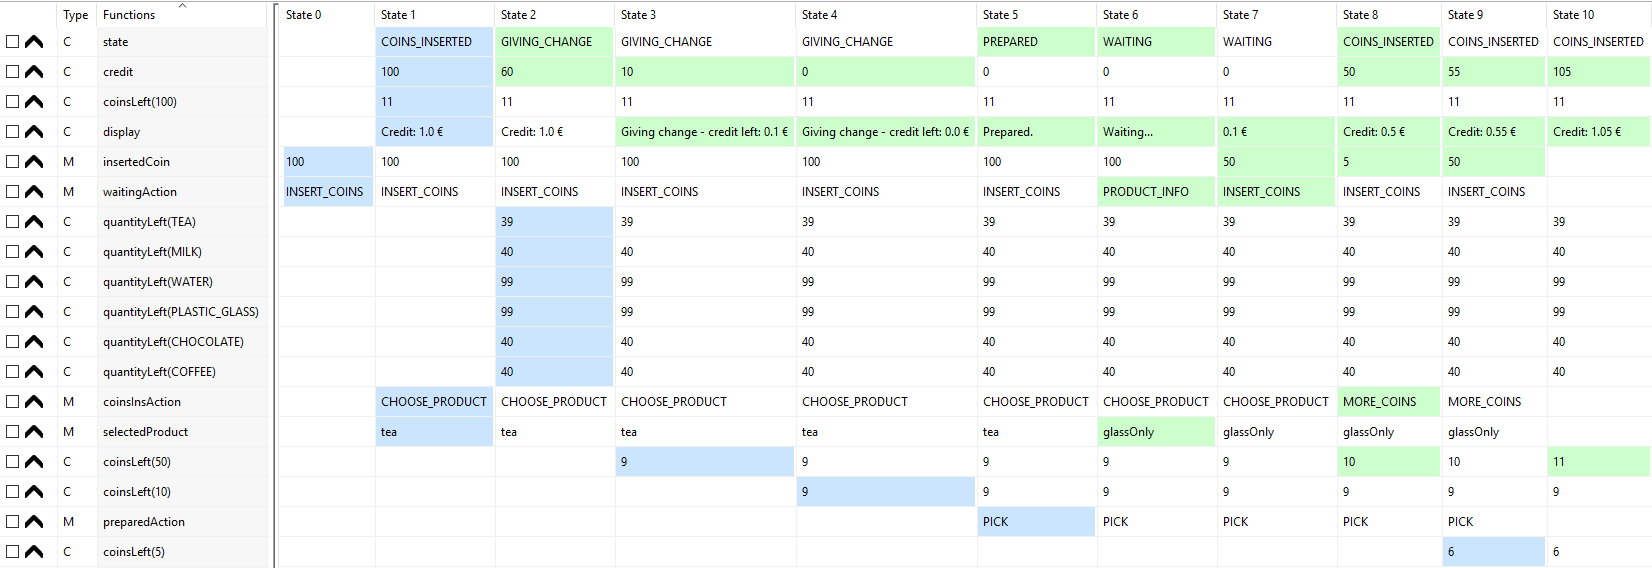
\includegraphics[width=1\textwidth]{Immagini/RandomRunASM.png}
	\caption{Test random ASM}
	\label{fig:randomExe}
\end{figure}

Nello specifico in figura ~\ref{fig:randomExe} si vede che, nella simulazione random abbiamo 10 stati in cui:
\begin{itemize}
	\item State0: inserita una moneta da 1€;
	\item State1: scelto come prodotto il \textit{the};
	\item State2: vengono diminuiti gli ingredienti utilizzati (1 TEA e 1 WATER) e viene dato il resto;
	\item State3: il the costa 0.4€, la macchinetta deve fornire un resto di 0.6€. Inizia erogando una moneta da 50 cent, e diminuisce il quantitativo di monete da 50 cent disponibili;
	\item State4: restano 10 cent di resto da dare. Fornisce quindi il resto e decrementa le monete da 10 cent disponibili;
	\item State5: il \textit{the} viene prelevato dall'utente;
	\item State6: la macchinetta si trova in uno stato di WAITING, e un utente chiede informazioni relativamente al solo bicchiere (GLASS ONLY);
	\item State7: mentre il display mostra il prezzo del bicchiere (0.1€), l'utente inserisce 50 centesimi;
	\item State8: l'utente inserisce altri 5 centesimi;
	\item State9: l'utente inserisce altri 50 centesimi;
	\item State10: terminazione random run.
\end{itemize}